\documentclass[a4paper,12pt]{scrartcl}
\usepackage{graphicx}
\usepackage[none]{hyphenat}
\usepackage{tikz}
\usepackage{amsmath}
\usepackage{pgfplots}

\usetikzlibrary{shapes}
\usetikzlibrary{arrows}
\usetikzlibrary{calc,positioning}

\def\labelitemi{--}

\pgfplotsset{compat=1.9} 

\begin{document}
\title{Classification Trees}
\subtitle{Data Mining 2015: assignment 1}
\author{Sebastiaan Jong (5546303) \& Bas Geerts (5568978)}
\date{}
\maketitle
\section{Introduction}
This report is written for the first assignment of the Data Mining (2015) course at Utrecht University. The goal of this assignment was to write a function in the R programming language that constructs a classification tree on a certain dataset, and to figure out efficient parameters for this tree.
\section{Data}
For this assignment we used the Heart Disease dataset from the University of California, Irvine machine learning repository. The preprocessed version for this assignment contains 297 instances and 14 attributes. The class label for this assignment is AHD, which indicates whether the patient has been diagnosed with a heart disease, the preprocessed dataset contains 137 instances where this is the case.

\section{Experiments}
The size of the classification tree is controlled by the \textit{nmin} (minimum internal node size) and \textit{minleaf} (minimum leaf size) parameters. Instead of brute forcing all possible values it is better to only try some sensible values and narrow down the optimal settings from there. It is possible to make a few observations regarding sensible parameter values (where \textit{n} is the dataset size): 
    \begin{itemize}
        \item Both $nmin$ and $minleaf$ should not be larger than $n/2$.
        \item The $minleaf$ parameter should not be larger than $nmin/2$. 
    \end{itemize}
The experiment uses a random trainingset of 200 rows from the initial dataset, the remaining 97 rows are used as testsample.
To quickly find an approximation of good parameter values, we tried all likely values for $nmin$ between 1 and 100 with a certain ratio to $minleaf$. The results are plotted in Figure 1, results are obtained by performing a 10-fold cross validation for each different parameter on the same trainingset. For example, the ratio 3:1 means that at $nmin = 45$, we tried $minleaf = 15$. The results from Figure 1 indicate that a well performing value for $nmin$ might be found between 10 and 20, since the error rate is consistently low at these points. 

    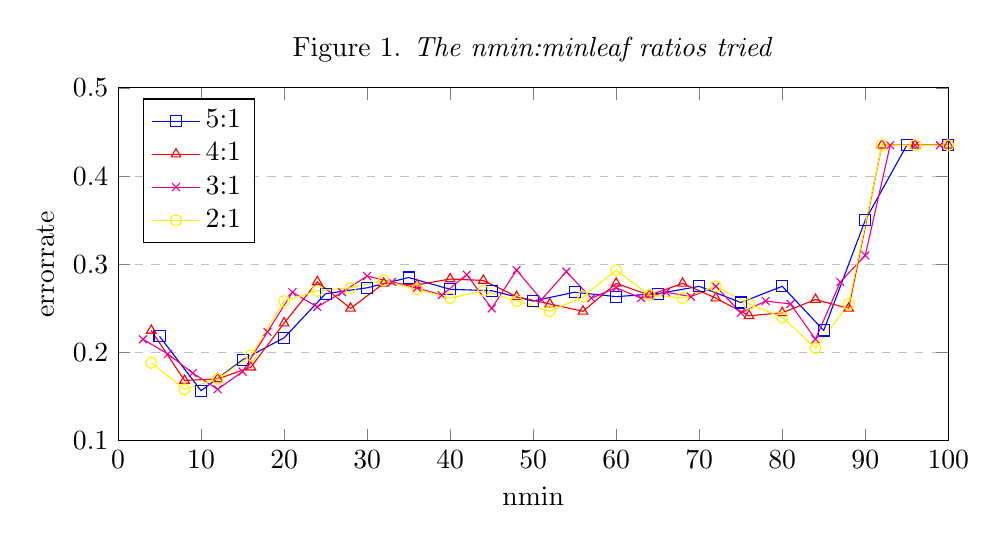
\begin{tikzpicture}
        \begin{axis}[
            title={Figure 1. \textit{The nmin:minleaf ratios tried}},
            xlabel={nmin},
            ylabel={errorrate},
            xmin=0, xmax=100,
            ymin=0.1, ymax=0.5,
            width=1\textwidth,
            height=0.5\textwidth,
            legend pos=north west,
            ymajorgrids=true,
            grid style=dashed
        ]
         
        \addplot[color=blue,mark=square,]
            coordinates {
                (5.0000000,0.2183333)(10.0000000,0.1566667)(15.0000000,0.1916667)(20.0000000,0.2166667)(25.0000000,0.2666667)(30.0000000,0.2733333)(35.000000,0.285000)(40.0000000,0.2716667)(45.000000,0.270000)(50.0000000,0.2583333)(55.0000000,0.2683333)(60.0000000,0.2633333)(65.0000000,0.2666667)(70.0000000,0.2750000)(75.0000000,0.2566667)(80.0000000,0.2750000)(85.0000000,0.2250000)(90.0000000,0.3500000)(95.0000000,0.4350000)(100.0000000,0.4350000)
            };
            \addlegendentry{5:1}

        \addplot[color=red,mark=triangle,]
            coordinates {
                (4.000000,0.225000)(8.0000000,0.1683333)(12.000000,0.170000)(16.0000000,0.1833333)(20.0000000,0.2333333)(24.000000,0.280000)(28.000000,0.250000)(32.0000000,0.2783333)(36.0000000,0.2766667)(40.0000000,0.2833333)(44.0000000,0.2816667)(48.0000000,0.2633333)(52.0000000,0.2550000)(56.0000000,0.2466667)(60.0000000,0.2783333)(64.0000000,0.2650000)(68.0000000,0.2783333)(72.0000000,0.2616667)(76.0000000,0.2416667)(80.0000000,0.2450000)(84.0000000,0.2600000)(88.0000000,0.2500000)(92.0000000,0.4350000)(96.0000000,0.4350000)(100.000000,0.435000)
            };
            \addlegendentry{4:1}
            
            \addplot[color=magenta,mark=x,]
                coordinates {
                    (3.000000,0.215000)(6.0000000,0.1983333)(9.0000000,0.1766667)(12.0000000,0.1583333)(15.0000000,0.1783333)(18.0000000,0.2233333)(21.0000000,0.2683333)(24.0000000,0.2516667)(27.0000000,0.2683333)(30.0000000,0.2866667)(33.000000,0.280000)(36.0000000,0.2733333)(39.000000,0.265000)(42.0000000,0.2883333)(45.000000,0.250000)(48.0000000,0.2933333)(51.0000000,0.2600000)(54.0000000,0.2916667)(57.0000000,0.2616667)(60.0000000,0.2733333)(63.0000000,0.2616667)(66.0000000,0.2683333)(69.0000000,0.2633333)(72.0000000,0.2750000)(75.0000000,0.2450000)(78.0000000,0.2583333)(81.0000000,0.2550000)(84.0000000,0.2150000)(87.0000000,0.2800000)(90.0000000,0.3100000)(93.00000,0.43500)(96.0000000,0.4350000)(99.0000000,0.4350000)
                };   
            \addlegendentry{3:1}

            \addplot[color=yellow,mark=o,]
                coordinates{
                    (4.0000000,0.1883333)(8.0000000,0.1583333)(12.000000,0.170000)(16.0000000,0.1966667)(20.0000000,0.2583333)(24.000000,0.270000)(28.0000000,0.2733333)(32.0000000,0.2816667)(36.0000000,0.2716667)(40.0000000,0.2616667)(44.0000000,0.2700000)(48.0000000,0.2583333)(52.0000000,0.2466667)(56.0000000,0.2633333)(60.0000000,0.2933333)(64.0000000,0.2650000)(68.0000000,0.2616667)(72.0000000,0.2750000)(76.0000000,0.2550000)(80.0000000,0.2400000)(84.0000000,0.2050000)(88.0000000,0.2550000)(92.0000000,0.4350000)(96.0000000,0.4350000)(100.0000000,0.4350000)
                };
            \addlegendentry{2:1}

        \end{axis}
    \end{tikzpicture}

    The results of performing another crossvalidation on all $nmin$ and $minleaf$ values where $nmin$ is between 10 and 20 with steps of 2 is shown in table 1. 

    \begin{center}
        \begin{tabular}{| l | l | l |}
        \hline
        $nmin$  & $minleaf$ & Errorrate & Nodes & Leafs & Construction time (sec)\\ \hline
            20 & 3275 & 170 \\ \hline
            25 & 3345 & 177 \\ \hline
            30 & 3364 & 173 \\ \hline
            35 & 3350 & 173 \\ \hline
            40 & 3378 & 178 \\ \hline
            45 & 3703 & 180 \\ \hline
            50 & 3617 & 179 \\ \hline
            55 & 3595 & 179 \\ \hline
            60 & 3595 & 179 \\ \hline
            65 & 3595 & 179 \\ \hline
        \end{tabular}
        ~\\
        ~\\
        Table 2: results of experiment 1.
    \end{center}

\tikzset{
  treenode/.style = {align=center, inner sep=0pt, text centered,
    font=\sffamily}
}

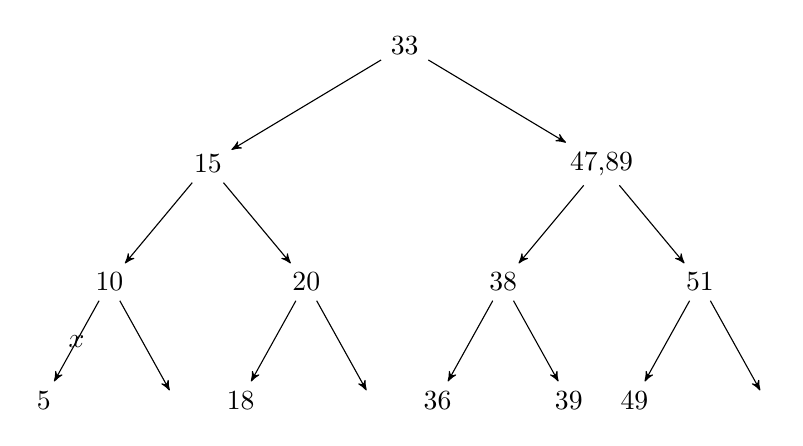
\begin{tikzpicture}[->,>=stealth',level/.style={sibling distance = 5cm/#1,
  level distance = 1.5cm}] 
\node {33}
    child{ node {15} 
            child{ node {10} 
                child{ node {5} edge from parent node[]
                         {$x$}} %for a named pointer
                            child{ node {}}
            }
            child{ node {20}
                            child{ node {18}}
                            child{ node {}}
            }                            
    }
    child{ node {47,89}
            child{ node {38} 
                            child{ node {36}}
                            child{ node {39}}
            }
            child{ node {51}
                            child{ node {49}}
                            child{ node {}}
            }
        }
; 
\end{tikzpicture}
\end{document}

\section{Results}





\end{document}